\section{Visualization}

The visualizations were done without the use of sampling on the dataset, hence all the below plots represent all the data points in the dataset.

Each sequence in the dataset contains different websites, represented by numbers, in a particular order. To understand what the most frequently visited websites are, each event(number) in a sequence is plotted against its count in the entire dataset in Fig. \ref{website_histogram}. From this plot, it is apparent that the first website, ``frontpage'' is visited far more frequently than any of the others and is most likely to be present in the final list of frequent sequences.

\begin{figure}[h]
    \centerline{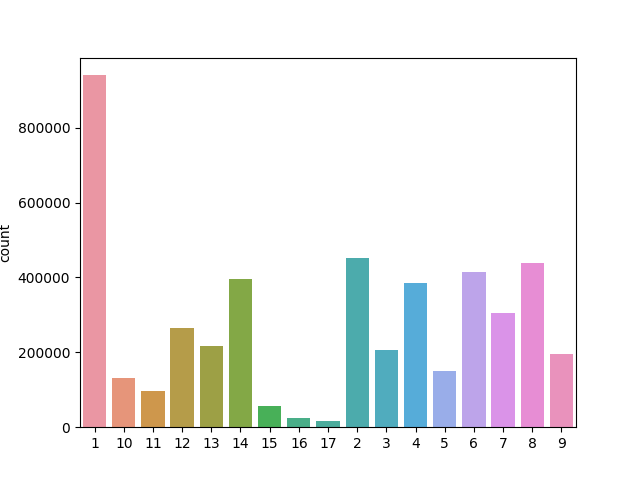
\includegraphics[width=0.5\textwidth]{figures/histogram_categories.png}}
    \caption{Plot showing number of times each website is visited}
    \label{website_histogram}
\end{figure}

The algorithm also depends on the length of each sequence and it is a good idea to know the distribution of sequence lengths in the dataset. The plot in Fig. \ref{distribution_lengths} shows the lengths of sequences in the dataset as a univariate distribution. Majority of the lengths are concentrated between 0 to 1000 with very few sequences having a length greater than 2000. The average of all the lengths in the dataset is 4.7 which can be seen from the figure with a huge portion of lengths concentrated just after 0.

\begin{figure}[h]
    \centerline{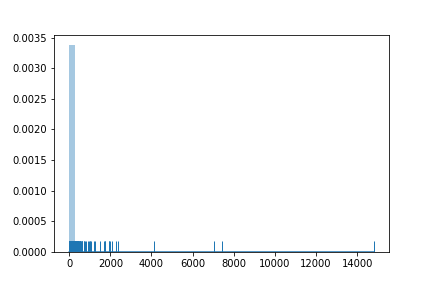
\includegraphics[width=0.5\textwidth]{figures/distribution_lengths.png}}
    \caption{Distribution of sequence lengths in the dataset}
    \label{distribution_lengths}
\end{figure}
